% !TEX root = ../main.tex

\subsection{Dipole Directivity using Dual Monopole Approach} \label{subsec:directivity}

The dual monopole method allows the investigation of the directivity patterns of a dipole. Sound directivity describes how the sound propagates in space due to the varying sound generation profiles at the source. This is highly relevant to the open rotor as the sound propagation from such system varies in space due the radiation profiles and kinematics.

Two standard tests are conducted, where the dipole is stationary and another that it moves at $u_x=10m/s$ to demonstrate the convective effects. The observers are set as a sphere located at a distance of $50m$, from the origin. In either case, the sources are aligned along the global y-axis at a distance $\delta=0.01/k$.

\begin{figure}[H]
    \centering
    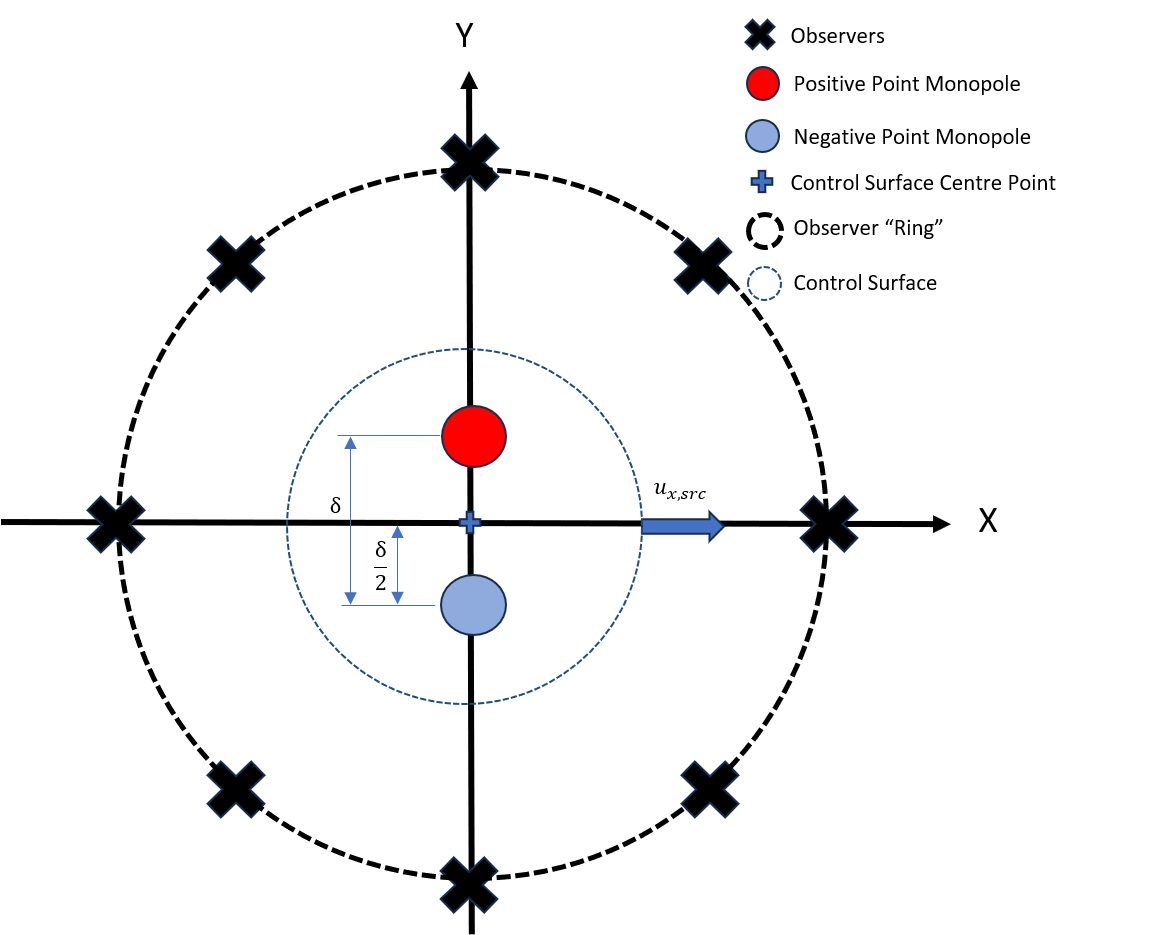
\includegraphics[width=0.8\linewidth]{fig_dipole/directivity_case.png}
    \caption{Test case for directivity}
    \label{fig:directivity_case}
\end{figure}

The stationary case show a standard directivity "figure-8" pattern, showing the locality of the individual monopoles. Imposing a translation to the source alters this pattern towards the $x$-axis as the source moves in said direction. It can be seen in either case that as the sound pressure along the x-axis is essentially 0. This is due to how the dipole itself is defined, where the two monopoles have equal and opposite signs, which causes the pressure along the x-axis to cancel.

\begin{figure}[H]
    \centering

    \begin{subfigure}[b]{0.45\textwidth}
        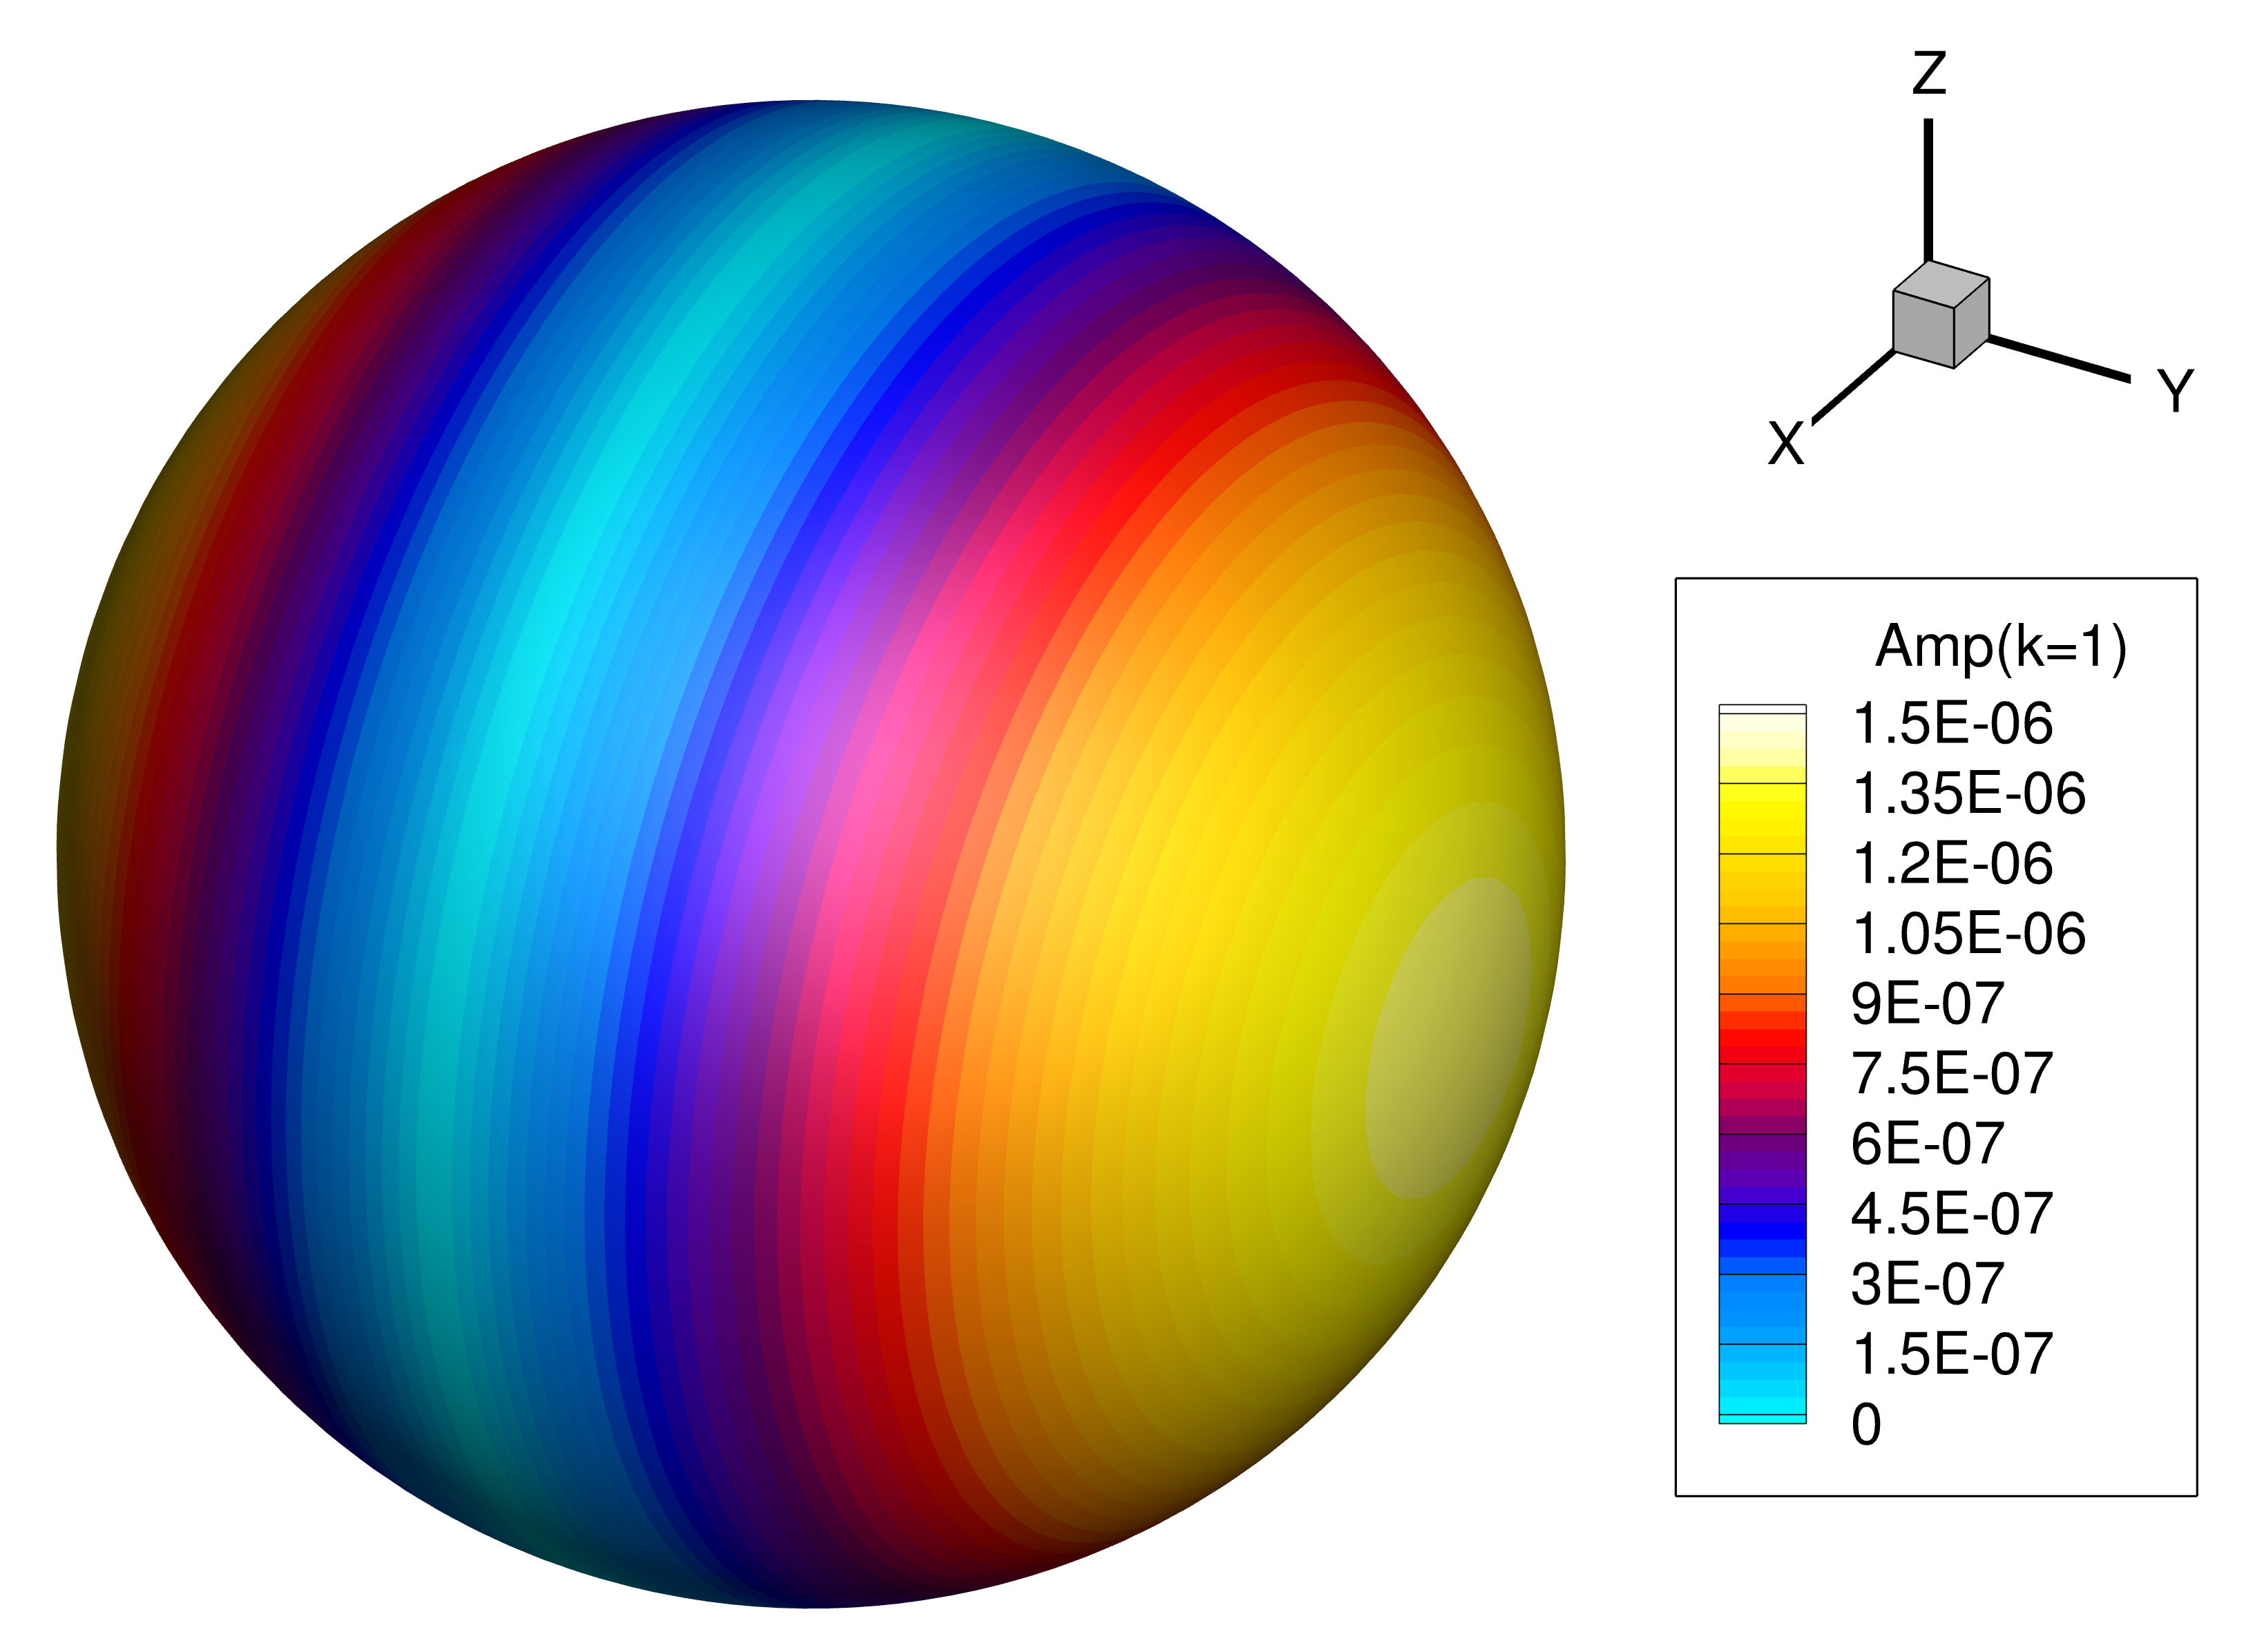
\includegraphics[width=\textwidth]{fig_dipole/directivity_stationary_3D.png}
        \caption{}
        \label{fig:directivity_stationary_3D}
    \end{subfigure}
    \hfill
    \begin{subfigure}[b]{0.45\textwidth}
        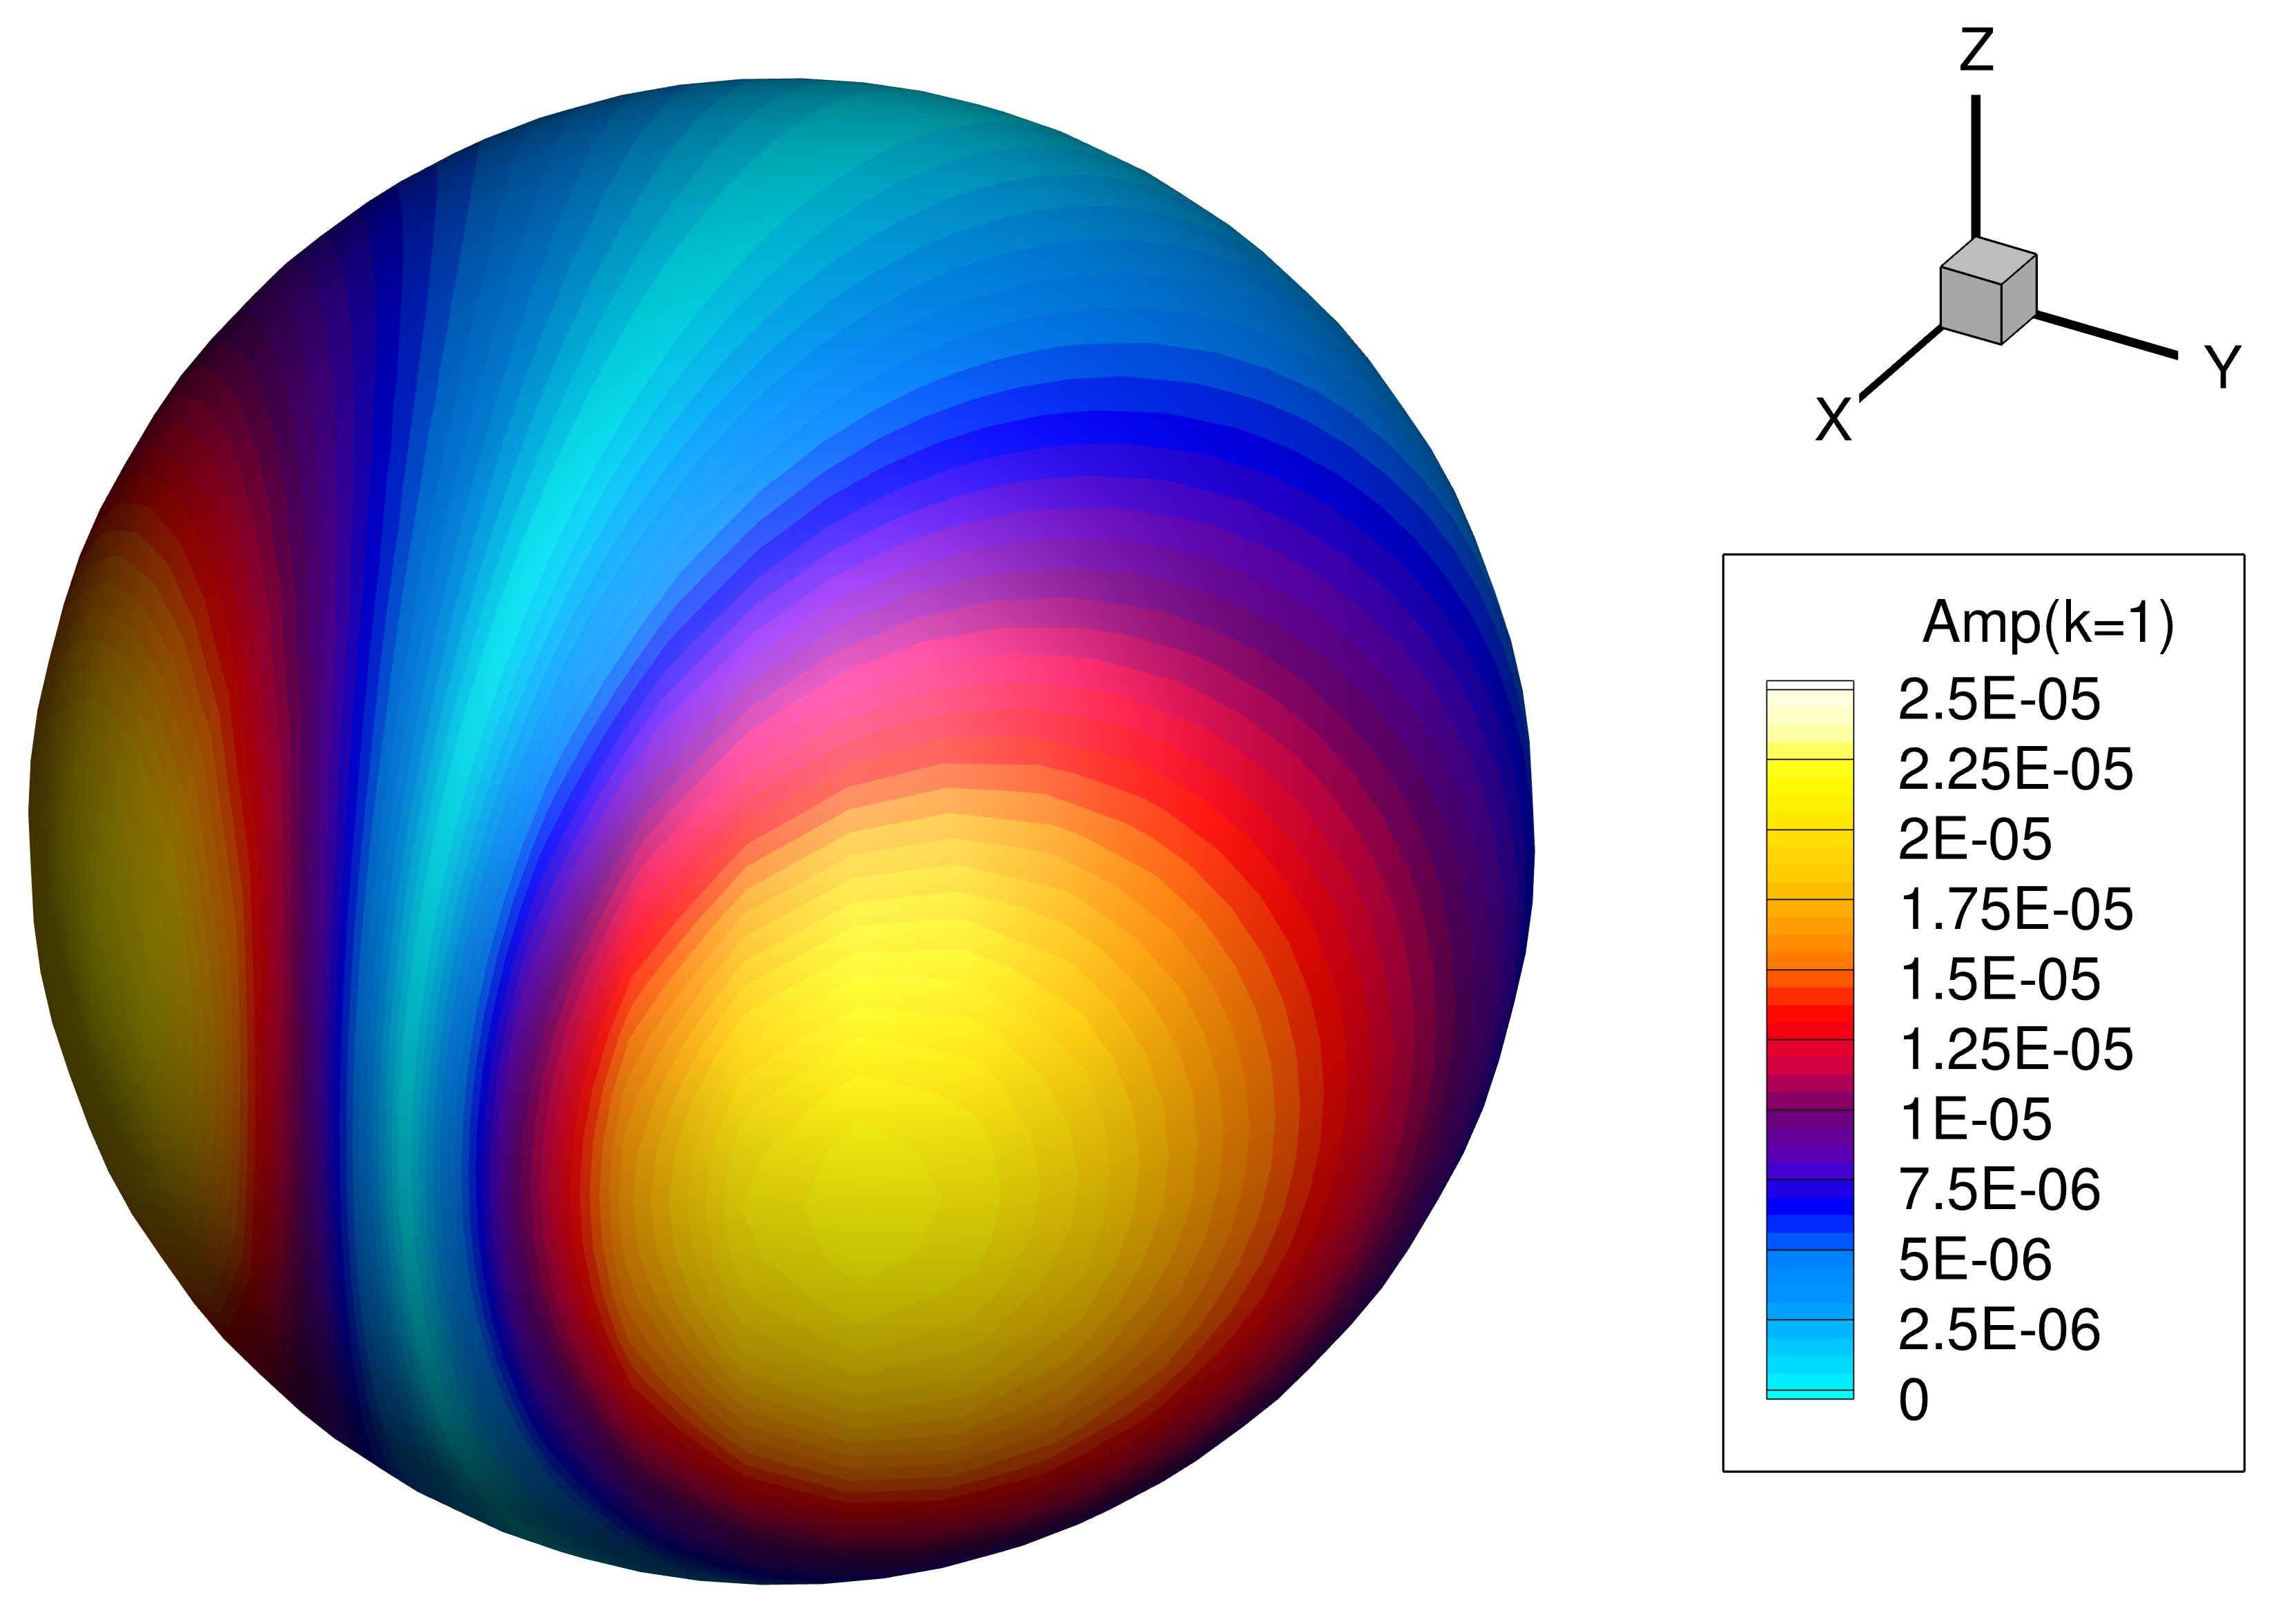
\includegraphics[width=\textwidth]{fig_dipole/directivity_translating_3D.png}
        \caption{}
        \label{fig:directivity_translating_3D}
    \end{subfigure}

    \vspace{0.25cm}
    
    \begin{subfigure}[b]{0.8\textwidth}
        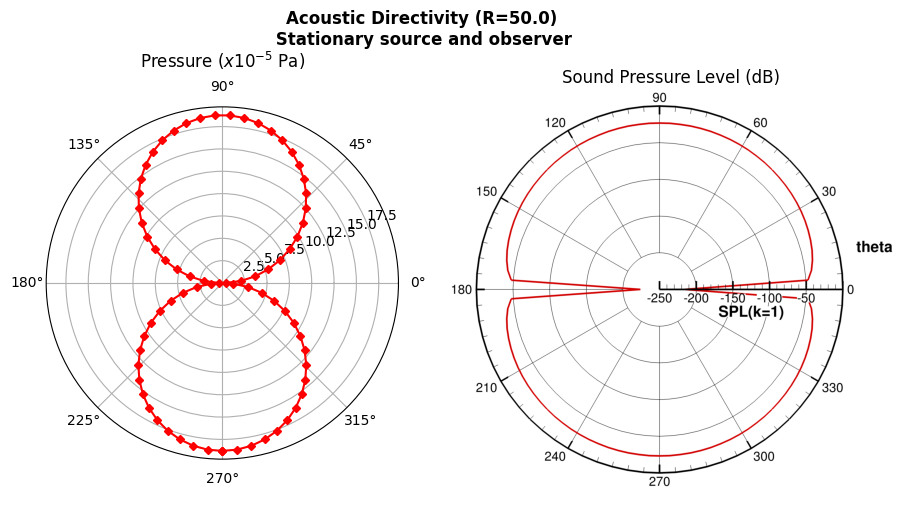
\includegraphics[width=\textwidth]{fig_dipole/directivity_stationary_new.png}
        \caption{}
        \label{fig:directivity_stationary_plot}
    \end{subfigure}

    \begin{subfigure}[b]{0.8\textwidth}
        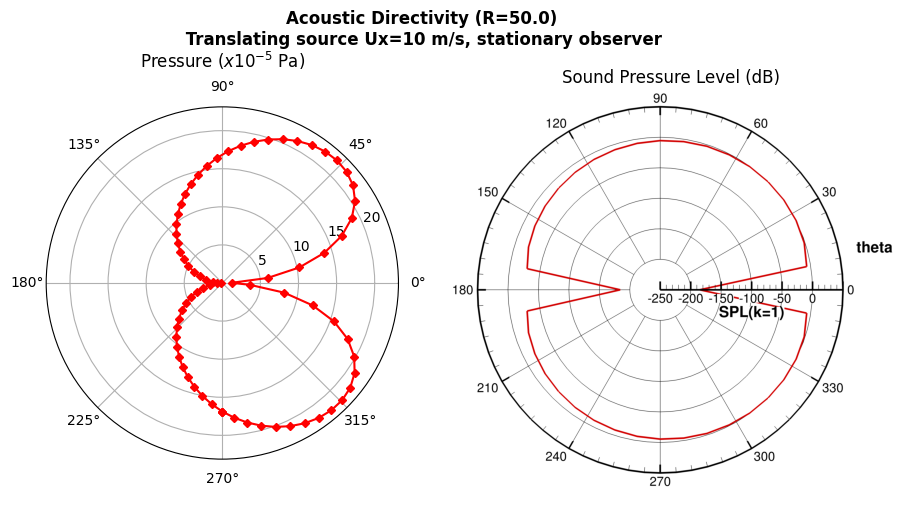
\includegraphics[width=\textwidth]{fig_dipole/directivity_translating_new.png}
        \caption{}
        \label{fig:directivity_translating_plot}
    \end{subfigure}

    \caption[Directivity of dual monopoles]{\centering Directivity of dual monopoles, stationary case with a) surface plot and c) polar plot; and translating case with b) surface plot and d) polar plot}
    \label{fig:directivity_stationary}
\end{figure}